\documentclass[10pt]{NSP1}
\usepackage{url,floatflt}
\usepackage{helvet,times}
\usepackage{graphics,graphicx}
\usepackage{mathptmx,amsmath,amssymb,bm}
\usepackage{float}
\usepackage[bf,hypcap]{caption}
\usepackage{booktabs}
\usepackage{array}
\usepackage{tabularx}
\usepackage[dvipsnames,table,xcdraw]{xcolor}

\addtolength{\oddsidemargin}{.5in}
\addtolength{\evensidemargin}{-.5in}

\tolerance=1
\emergencystretch=\maxdimen
\hyphenpenalty=10000
\hbadness=10000

\topmargin=0.00cm

\def\sm{\smallskip}
\def\no{\noindent}

\def\firstpage{1}
\setcounter{page}{\firstpage}
\def\thevol{7}
\def\thenumber{1}
\def\theyear{2026}


\begin{document}

\titlefigurecaption{{\large \bf \rm Applied Mathematics \& Information Sciences}\\
{\it\small An International Journal}}

\title{Machine Learning-Based Prediction of Particle Size in PLGA Nanoparticle Formulations}

\author{Hamza Abu Owida\hyperlink{author1}{$^1$},
      Areen Arabiat\hyperlink{author2}{$^2$},
        Jaber A. Alwidian\hyperlink{author3}{$^3$}
        Hamza A. Mashagba \hyperlink{author4}{$^4$}
        Asokan Vasudevan\hyperlink{author5}{$^5$},
        Azlan B. Abd Aziz\hyperlink{author7}{$^{4,*}$},
        Mohammad Faleh Ahmmad Hunitie\hyperlink{author6}{$^6$},  Suleiman Ibrahim Mohammad\hyperlink{author8}{$^{7,8}$}} 
 
\institute{%
$^1$Medical Engineering Department, Faculty of Engineering, Al-Ahliyya Amman University, Amman 19111, Jordan\\
$^2$Department of Communications and Computer Engineering, Faculty of Engineering, Al-Ahliyya Amman University, Amman 19111, Jordan,
$^3$Department of Data Science and Artificial intelligence, Faculty of Information Technology, Applied Science Private University, Amman 11931, Jordan\\
$^4$Faculty of Engineering and Technology, Multimedia University, Centre for Wireless Technology (CWT), Cyberjaya, Selangor 63100,
Malaysia\\
$^5$Faculty of Business and Communications, INTI International University,  Negeri Sembilan 71800, Malaysia\\
$^6$Department of Public Administration, School of Business, University of Jordan, Amman 11942, Jordan\\
$^7$Department of Business Administration, School of Business, Al al-Bayt University, Mafraq 25113, Jordan\\
$^8$Research follower, INTI International University, 71800 Negeri Sembilan, Malaysia
}

\titlerunning{ML-Based Prediction of PLGA Nanoparticle Particle Size}
\authorrunning{Azlan B. Abd Aziz}

\mail{ azlan.abdaziz@mmu.edu.my}

\received{15 Jan. 2026}
\revised{2 Apr. 2026}
\accepted{6 Jun. 2026}
\published{15 Jun. 2026}

\abstracttext{Poly lactic-co-glycolic acid (PLGA) nanoparticles' particle size is a crucial quality
parameter, but precise pre-experimental prediction is still challenging since it depends on coupled
polymer, drug, and formulation variables across heterogeneous investigations. Hydrodynamic particle
size was modeled in this study using a carefully selected literature-derived dataset that included
430 formulations from 59 literature references and 15 predictors. Nevertheless, the suggested model
shows very little cross-study generality. Drug hydrogen-bond acceptor count (\textit{mol\_Hacceptors}),
LA/GA ratio, surfactant concentration, drug/polymer ratio, drug lipophilicity, and polymer molecular
weight were consistently found to be the main predictors of particle size by interpretable machine
learning (ML) analyses, with distinct non-linear and interaction-dependent behavior. A grouped
external hold-out split at the literature-reference level and random 5-fold cross-validation were
used to assess the performance of the proposed model. While performance declined on the external
reference-level test set (RMSE\,=\,61.56\,nm, MAE\,=\,49.63\,nm, $R^2$\,=\,0.18), random 5-fold
cross-validation demonstrated good apparent in-distribution performance
(RMSE\,=\,49.75\,nm, MAE\,=\,26.63\,nm, $R^2$\,=\,0.76). These results demonstrate that
study-aware external validation is necessary prior to widespread predictive implementation, but they
also support the use of interpretable machine learning for formulation screening and hypothesis
creation.}

\keywords{Machine Learning; Cross-Validation; poly lactic-co-glycolic acid; formulation; biomedical}

\maketitle

%----------------------------------------------------------------------
\section{Introduction}
%----------------------------------------------------------------------

As an approach to drug delivery, PLGA (poly lactic-co-glycolic acid) nanoparticles have been
utilized extensively due to their biodegradable nature, biocompatible properties and their ability
to be modified physically and chemically~\cite{ref1,NEW1}. The production of these nanoparticles can be
accomplished at scale by utilizing a variety of methods for polymerization; therefore, researchers
can systematically modify the physical characteristics of the polymers, including the ratios of
lactic and glycolic acid, molecular weights, and chemical compositions of the end-groups, along
with various formulation and processing factors, to enable the fine-tuning of the rates of
degradation of the polymer and the release of drugs, enhance the stability of fragile
pharmaceutical products and allow for the administration of the drugs via multiple routes~\cite{ref2,NEW2}.
Furthermore, PLGA has had a documented history of being accepted by regulatory bodies for use in
the controlled release of pharmaceutical products, such as long-acting depot formulations, which
demonstrates the translation of this material into a viable candidate for the development of
advanced nanomedicine~\cite{ref2,ref3}.

Researchers throughout the biomedical community continue to explore the utilization of PLGA
nanoparticles to encapsulate small molecules, biologics, nucleic acids, and imaging agents, as well
as to surface-engineer them with techniques such as PEGylation and/or the attachment of ligands to
modulate their biodistribution, cellular interaction and therapeutic index~\cite{NEW3,ref4}.

Particle size is one of the critical parameters that affect the performance of PLGA nanoparticles.
Particle size influences the colloidal stability, drug loading and release, diffusion and transport
across physiological barriers, and interactions with immune surveillance pathways, which subsequently
impact the pharmacokinetics and efficacy of therapy~\cite{ref5,ref6,NEW4}. Therefore, the size of
nanoparticles, as well as their shape and surface chemistry, affect the mechanisms of cellular
uptake and organ level distribution of the drug carrier, leading to the necessity to strictly
control both the size and polydispersity of nanoparticles during both research and
manufacturing~\cite{ref7,ref8,NEW5}.

However, it is difficult to produce nanoparticles of a predetermined size with good
reproducibility. PLGA nanoparticles are formed through tightly coupled, nonlinear processes that
include solvent--antisolvent mixing, supersaturation-induced nucleation and growth of polymer
particles, precipitation of polymer, and stabilization of polymer particles through surfactants,
which collectively respond to changes in the formulation and processing variables of the fabrication
route~\cite{ref9,ref10}. Many fabrication routes for PLGA nanoparticles, such as nanoprecipitation
and emulsion-based techniques, involve numerous process variables that interact with each other in
a complex manner and often in a non-intuitive fashion, leading to considerable batch-to-batch
variability~\cite{ref11,ref12}. Although microfluidic platforms provide better control over the
mixing process and reproducibility, they also add additional process variables, such as the
architecture of the channels, the ratio of the flow rate, and the residence time, further increasing
the complexity of the design space, and emphasizing the need for systematic, data-driven strategies
to optimize the formulation of nanoparticles~\cite{ref13,ref14}.

Optimization of PLGA nanoparticles has largely employed either one-factor-at-a-time experimentation
or statistically based methodologies, primarily the Design of Experiments (DoE), which is part of
the Quality by Design (QbD)/DoE paradigm~\cite{ref15}. While QbD/DoE provides an efficient method
to identify local factor effects and interactions, many practical aspects of developing nanoparticles
increasingly present researchers with sparse datasets, heterogeneous protocols among different
studies, and high dimensional parameter spaces that are expensive and time-consuming to evaluate
experimentally~\cite{ref10,ref12}. As a result, there is increasing interest in the application of
ML as a supplementary methodology to learn complex structure-process-property relationships directly
from experimental data to facilitate improved predictions and more efficient formulation
development~\cite{ref16,ref17}. Within the larger scope of nanomedicine, workflows guided by ML
have shown value in navigating large combinatorial formulation landscapes, combining high-throughput
experimentation with iterative model-driven refinement, and optimizing target biological endpoints,
such as cellular uptake~\cite{ref18}. Simultaneously, recent studies on PLGA nanoparticle synthesis
have demonstrated the capability of ML-based regression frameworks to accurately predict the sizes
(and, in certain instances, zeta potentials) of PLGA nanoparticles, providing evidence that
ML-based rational design and process optimization may be applied to PLGA nanoparticle
synthesis~\cite{ref19,ref20}.

Although many challenges remain to implement ML in the design of PLGA nanoparticles, the two
biggest problems are predictive robustness, which is typically influenced by relatively low sample
numbers, variations in protocol among samples, and shifts in data sets that increase an ML
algorithm's susceptibility to overfitting, and therefore potentially degrade its performance when
it is used on new formulations, equipment, or manufacturing settings~\cite{ref16,ref17}. Another
significant problem is lack of validation and the relative lack of interpretability that constrains
both scientific and regulatory confidence: formulation scientists must have the ability to obtain
reliable predictions, and in addition to that they need to understand what formulation and
processing parameters drove those predictions so that they could modify those parameters in order
to produce a particle of a desired size~\cite{ref21,ref22}. Both of these problems will be solved
if researchers follow established guidelines and best practices in developing their ML algorithms,
i.e., leakage-free pre-processing, principled hyper-parameter search, and performance evaluation
that is aligned with the way the ML model will ultimately be used, and include validation that
tests the ML model's ability to generalize~\cite{ref23}. Additionally, cross-validation, especially
cross-validation that takes into account the structure of the experiments, provides a robust
estimate of performance of the ML model based upon internal data, whereas external validation using
independent data sets or experimental protocols provides a very strict test of whether or not the
ML model can be transferred to other conditions~\cite{ref24,ref25,ref26}. Finally, improvements in
Explainable AI provide the opportunity for systematic exploration of how the ML model behaves; for
example, feature-attribution methods (for example, methods based on Shapley-values) allow
identification of the most influential formulation and processing factors and interactions between
them that are consistent with an understanding of the mechanisms behind nanoprecipitation and
emulsification~\cite{ref22,ref23}.

The aim of this study was to develop a literature-derived, study-aware ML workflow for predicting
the particle size of PLGA nanoparticles from formulation descriptors, while explicitly accounting
for heterogeneity across independent studies. In addition to model development, the study
systematically compares conventional random cross-validation, which primarily reflects
in-distribution performance, with reference-level external testing that evaluates the model's
ability to generalize across different literature sources. This design enables a more realistic
assessment of predictive performance and highlights the impact of study-level variability on model
reliability.

%----------------------------------------------------------------------
\section{Materials and Methods}
%----------------------------------------------------------------------

\subsection{Study Design and Data Sources}

This study developed and evaluated predictive models for the hydrodynamic diameter of PLGA
nanoparticles using a custom-curated, literature-derived formulation dataset. Records were retained
only when hydrodynamic particle size and the required formulation descriptors were reported
sufficiently for structured extraction, and duplicate formulations or repeated measurements were
consolidated at the formulation level before modeling~\cite{ref23}.
\begin{figure*}
    \centering
    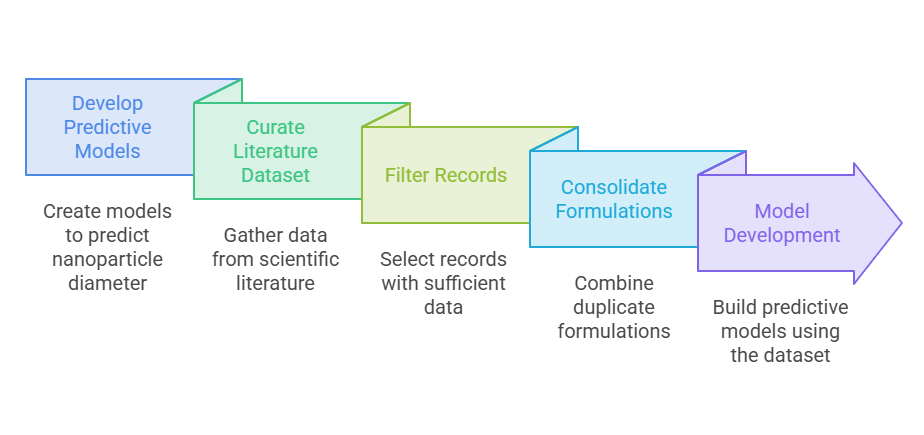
\includegraphics[width=1\linewidth]{Vvisual selection.png}
    \caption{The proposed work}
    \label{ff}
\end{figure*}
The final modeling population consisted of 430 unique formulations obtained from 59 separate
literature references. Each formulation was assigned a Literature Reference Identifier so that
data splitting could be performed at the study level, thereby limiting leakage of study-specific
information between development and test partitions and enabling a more realistic assessment of
out-of-study prediction. This modeling dataset was custom-curated for the present study and is not
identical to the broader Mendeley PLGA nanoparticle data record. Table~\ref{tab1} summarizes
dataset composition and the exact development/external split used for evaluation, as shown in Figure \ref{ff}.

\begin{table*}[t]
\caption{Summary of dataset composition and external reference-split evaluation.}
\label{tab1}
\centering
\small
\begin{tabular}{lccc}
\toprule
\textbf{Dataset component} & \textbf{References} & \textbf{Formulations} & \textbf{Notes}\\
\midrule
Total curated dataset & 59 & 430 & All unique formulations retained for modeling\\
Model-development set & 47 & 350 & Used for fitting and internal cross-validation\\
External reference-split test set & 12 & 80 & No literature references shared with development set\\
Predictor set & -- & 15 & Polymer, drug, surfactant, solvent, and phase-ratio descriptors\\
\bottomrule
\end{tabular}
\end{table*}

\subsection{Definitions and Preprocessing of Features}

Each formulation was described by 15 features spanning polymer, drug, surfactant, solvent, and
phase-ratio descriptors. These included polymer molecular weight, copolymer composition (LA/GA),
drug physicochemical descriptors (for example \textit{mol\_logP}, \textit{mol\_TPSA},
\textit{mol\_Hacceptors}, \textit{mol\_heteroatoms}, and \textit{mol\_melting\_point}), and
formulation descriptors such as drug/polymer ratio, surfactant concentration,
\textit{surfactant\_HLB}, aqueous/organic ratio, pH, and solvent-related variables. The full
predictor dictionary is provided in Table~\ref{tab2}.

\begin{table*}
\caption{Features dictionary used for the literature-derived PLGA nanoparticle model.}
\label{tab2}
\centering
\small
\begin{tabular}{p{2.8cm}p{2.2cm}p{3.2cm}p{4.5cm}}
\toprule
\textbf{Feature} & \textbf{Unit/Type} & \textbf{Encoding/Derivation} & \textbf{Scientific Rationale}\\
\midrule
polymer\_MW & Mol.\ weight & Numeric, as reported & Captures chain length, viscosity, and precipitation behavior\\
LA/GA & Lactide:glycolide ratio & Numeric ratio & Reflects polymer composition, hydrophobicity, and chain packing\\
polymer\_endgroup & Categorical & Curated polymer descriptor & May influence polymer polarity and interfacial behavior\\
mol\_logP & Dimensionless & Drug physicochemical descriptor & Represents lipophilicity and phase partitioning tendency\\
mol\_TPSA & \AA$^2$ & Drug physicochemical descriptor & Captures polarity and hydrogen-bonding-related transport behavior\\
mol\_Hacceptors & Count & Calculated molecular descriptor & Represents drug hydrogen-bond acceptor capacity\\
mol\_heteroatoms & Count & Calculated molecular descriptor & Summarizes polar atom content and interaction potential\\
mol\_melting\_point & $^\circ$C & Drug physicochemical descriptor & Proxy for crystal lattice strength and solvation behavior\\
drug/polymer & Ratio & Numeric formulation ratio & Controls relative solute loading during particle formation\\
surfactant\_concentration & Concentration & Numeric, as reported & Affects stabilization and interfacial coverage\\
surfactant\_HLB & Dimensionless & Surfactant descriptor & Reflects surfactant balance and emulsification tendency\\
aqueous/organic & Phase ratio & Numeric ratio & Represents solvent--antisolvent environment during precipitation\\
pH & Unitless & Coded/curated aqueous-phase descriptor & Can affect ionization and colloidal stabilization\\
solvent\_identity & Categorical & Organic-solvent descriptor & Captures solvent-specific effects on miscibility and evaporation\\
solvent\_polarity\_index & Dimensionless & Curated solvent descriptor & Represents solvent polarity and mixing behavior\\
\bottomrule
\end{tabular}
\end{table*}

Prior to modeling, exact duplicates were removed so that repeated formulations would not
disproportionately weight the fitted models. There were no missing values in the final feature
matrix; therefore, no imputation was required. Because the particle-size distribution was
right-skewed, the outcome was modeled on the logarithmic scale as $y = \log_{10}(\mathrm{PS_{nm}})$,
where $\mathrm{PS_{nm}}$ denotes hydrodynamic particle size in nanometers. Predictions were
back-transformed as $\widehat{\mathrm{PS}}_{\mathrm{nm}} = 10^{\hat{y}}$ for performance reporting
and prediction-versus-actual visualization.

\subsection{Supervised Machine Learning Workflow}

A Random Forest (RF) regression framework was selected as the main model because particle size
depends on nonlinearly coupled formulation effects~\cite{ref27,ref28,ref29}. RF can capture
non-linear interactions without pre-specification, and the fitted ensemble supports complementary
interpretability analyses including permutation importance, SHAP, and partial dependence plots.
The final RF model used 400 trees ($n\_\mathrm{estimators} = 400$), $\mathrm{max\_features} =
\texttt{`sqrt'}$, $\mathrm{min\_samples\_split} = 2$, $\mathrm{min\_samples\_leaf} = 1$,
$\mathrm{bootstrap} = \mathrm{True}$, and $\mathrm{random\_state} = 42$; all other parameters
were left at their default settings. These settings were selected to balance predictive stability
and ensemble diversity, thereby reducing correlation among trees and improving generalization. The
baseline comparator was a dummy regressor that predicted the training-set mean, and a
validation-curve analysis of $n\_\mathrm{estimators}$ was utilized to investigate the impact of
ensemble size independently.

\subsection{Training, Cross-Validation, and External Reference-Split Testing}

Two complementary validation regimens were used. The external reference-split evaluation is the
primary basis for claims of model generalizability in this study since random cross-validation
estimates in-distribution performance \cite{ref30,ref31}.

\begin{itemize}
\item \textbf{Random 5-fold cross-validation (CV):} standard shuffled 5-fold cross-validation was
used to estimate in-distribution performance. Out-of-fold predictions were generated for all
samples to construct prediction-versus-actual plots.
\item \textbf{External reference-split evaluation:} a grouped hold-out test split was created at
the literature-reference level such that no references were shared between training and test sets.
The external split comprised 12 references and 80 formulations, whereas model development used the
remaining 47 references and 350 formulations. The external test set was created using a grouped
random split at the literature-reference level with a fixed random seed ($\mathrm{random\_state} =
42$). This split was performed once and was not repeated.
\end{itemize}

This design explicitly distinguishes performance under conventional random splitting from
performance under cross-study domain shift.

\subsection{Performance Metrics}

Performance was quantified on back-transformed particle sizes (nm) using root mean squared error
(RMSE), mean absolute error (MAE), and coefficient of determination ($R^2$) ~\cite{ref32,ref33,ref34}. For random 5-fold
cross-validation, pooled out-of-fold metrics are reported together with fold-wise RMSE behavior in
the validation-curve analysis; external reference-split results are reported as held-out test-set
point estimates.

Root mean squared error (RMSE) is a measure of the average prediction error in the same units as
the target variable, calculated as the square root of the average of the squared discrepancies
between predicted and observed values as shown in Equation~(\ref{eq1})~\cite{ref27}:
\begin{equation}\label{eq1}
\mathrm{RMSE} = \sqrt{\frac{1}{n}\sum_{i=1}^{n}\left(y_i - \hat{y}_i\right)^2}
\end{equation}

Mean absolute error (MAE) is a measure of the average size of prediction mistakes, independent of
their direction, and is calculated by averaging the absolute disparities between projected and
actual values as shown in Equation~(\ref{eq2})~\cite{ref30}:
\begin{equation}\label{eq2}
\mathrm{MAE} = \frac{1}{n}\sum_{i=1}^{n}\left|y_i - \hat{y}_i\right|
\end{equation}

Coefficient of determination ($R^2$) measures the percentage of the observed data's variance that
the prediction model can account for, as shown in Equation~(\ref{eq3})~\cite{ref31}:
\begin{equation}\label{eq3}
R^2 = 1 - \frac{\displaystyle\sum_{i=1}^{n}\left(y_i - \hat{y}_i\right)^2}
                {\displaystyle\sum_{i=1}^{n}\left(y_i - \bar{y}\right)^2}
\end{equation}

The validation-curve analysis summarized fold-wise RMSE distributions across cross-validation folds
for varying estimator settings.

\subsection{Interpretability and Robustness Analyses}

To ensure interpretability and mitigate reliance on a single explanation method, three
complementary approaches were used:
\begin{itemize}
\item Permutation feature importance was computed on the external test set as the increase in RMSE
on the $\log_{10}$ scale after shuffling each feature repeatedly. Larger increases indicate greater
reliance of the fitted model on that feature for out-of-study prediction.
\item SHAP (TreeSHAP) values were computed to characterize the magnitude and direction of each
feature's contribution to predictions at the sample level and summarized using a global beeswarm
plot.
\item Partial dependence plots (PDPs) were used to visualize average marginal associations of
selected predictors with the fitted model output, while SHAP dependence plots were used to examine
directionality and interaction structure for dominant drivers. These plots describe model behavior
and should not be interpreted causally.
\end{itemize}

\subsection{Software and Reproducibility}

All analyses were conducted in Python using standard ML and scientific-computing libraries with
fixed random seeds for reproducibility. Evaluation used a leakage-resistant workflow, including
group-aware splitting at the literature-reference level for the external test. The curated dataset
and analysis code are available upon reasonable request.

%----------------------------------------------------------------------
\section{Results}
%----------------------------------------------------------------------

The curated dataset comprised 430 unique PLGA nanoparticle formulations described by 15 feature
variables. Observed particle sizes ranged from 20.2 to 1012.0\,nm (median\,=\,167.3\,nm;
IQR\,=\,138.6--210.8\,nm). Because the distribution was right-skewed, particle size was modeled
on the $\log_{10}$ scale and back-transformed to nanometers for reporting.

For external reference-split testing, 80 formulations from 12 literature references were held out
as the test set, while the remaining 350 formulations from 47 references were used for model
development. Table~\ref{tab1} summarizes dataset composition and the development of external split.
Under external reference-split evaluation, predictions were compressed toward intermediate values:
smaller particles were systematically overpredicted and larger particles were systematically
underpredicted, consistent with shrinkage toward the center of the training distribution.

Nevertheless, the RF still had some measurable signal above and beyond the baseline predictor:
\begin{itemize}
\item Baseline (mean predictor): RMSE\,=\,68.14\,nm, MAE\,=\,57.26\,nm, $R^2$\,=\,$-0.01$
\item Random Forest: RMSE\,=\,61.56\,nm, MAE\,=\,49.63\,nm, $R^2$\,=\,0.18
\end{itemize}



Under random 5-fold cross-validation, out-of-fold predictions clustered near the identity line in
the central region of the size distribution, with larger errors toward the extremes. In pooled out-of-fold terms, the RF model achieved
RMSE\,=\,49.75\,nm, MAE\,=\,26.63\,nm, and $R^2$\,=\,0.76.

These results demonstrate that strong apparent performance under random CV does not fully translate
to cross-study prediction, consistent with the presence of unmeasured study-specific variability.



Permutation importance was calculated on the external test set as the increase in RMSE
($\log_{10}$ scale) after repeated shuffling of each feature. Larger values indicate greater
reliance of the fitted model on that feature for external predictions. \textit{mol\_Hacceptors}
and LA/GA produced the largest RMSE increases, identifying them as the strongest predictors under
the more stringent out-of-study evaluation. On the other hand,
SHAP analysis showed a broadly similar ranking of dominant predictors while additionally revealing
the direction and sample-level magnitude of each feature's contribution.  Agreement between permutation importance and SHAP supports internal
consistency of the fitted model's explanations, but it should not be interpreted as evidence of
causal mechanism.



The depicts little variation of model performance across the tested ensemble sizes
($n\_\mathrm{estimators} = 50, 100, 200, 400, 800$); mean cross-validation RMSE changed only
modestly and the fold-wise RMSE distributions overlapped substantially, indicating that performance
in this setting was not highly sensitive to the number of trees. An ensemble size around 400 trees
therefore represented a reasonable operating point.



The PDPs  show average marginal effects on the model output on the
$\log_{10}$ scale. Rug plots indicate data density across the observed feature range, so trends in
sparse regions should be interpreted cautiously. Together, the PDPs provide further evidence of
non-linear relationships:
\begin{itemize}
\item LA/GA: increasing effect on model output up to an intermediate regime followed by a plateau.
\item Surfactant concentration: rapid change at low concentrations with diminishing marginal effect
at higher levels.
\item Polymer molecular weight: a threshold-like rise at low to moderate values followed by
stabilization.
\end{itemize}



The SHAP dependence plot for LA/GA within the fitted model demonstrated a
positive directional association, with higher LA/GA values often associated with larger anticipated
particle sizes. The color gradient indicates interaction with the surfactant regime, and the
discrete grouping represents frequently used formulation parameters. Model behavior, not mechanism,
is described by these relationships.


A SHAP dependence plot for \textit{mol\_Hacceptors} indicated a structured and
nonlinear association. For drugs having low acceptor numbers, SHAP values were positive and
indicated increased predicted sizes. Drugs having intermediate to high acceptor counts typically
showed negative SHAP values indicating decreased predicted sizes. Color mapping based on surfactant
concentrations indicated that the magnitude of the drug-descriptor effect was variable under
different surfactant conditions, which is consistent with coupled-model associations.
\textit{Mol\_Hacceptors} refers to the calculated total count of hydrogen-bond acceptor atoms
within a drug molecule.

\begin{figure*}[h]
\centering
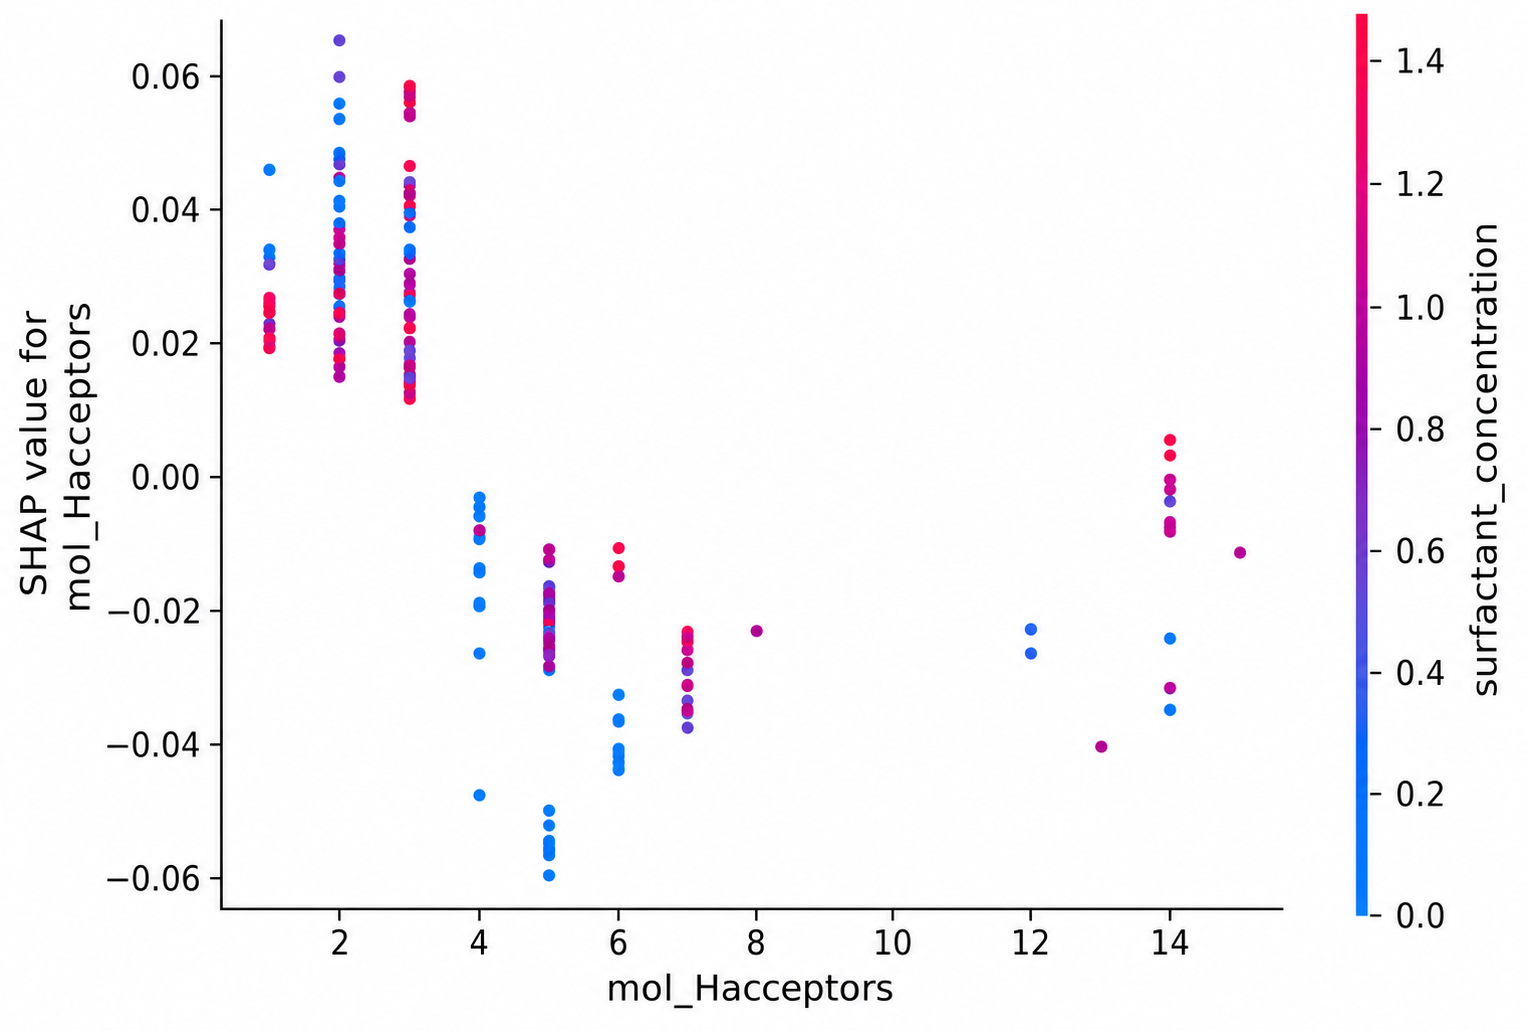
\includegraphics[width=0.75\linewidth]{fig7.png}
\caption{SHAP dependence plot for mol\_Hacceptors colored by surfactant concentration.}
\label{fig7}
\end{figure*}

Together, these analyses indicate that particle size in this literature-derived dataset is
influenced by non-linear relationships across polymer composition, surfactant conditions, and
drug polarity-related descriptors.

%----------------------------------------------------------------------
\section{Discussion}
%----------------------------------------------------------------------

The major challenge with literature-based formulation models is how often one finds domain shift
for each individual study. The way formulations are prepared, the rate at which solutions are
injected into the solution stream, whether additional components are added to the solution stream
in order to help mix and/or provide some form of mechanical shearing, etc., are all things that
can cause differences in what is measured as an average diameter but cannot be predicted based on
our current descriptor set. As such, cross-validation can predict too high of a deployable
performance if two samples from the same original literature study end up being used in both the
training and the testing folds.

Even though the external performance was reduced, the interpretability analyses showed that
\textit{mol\_Hacceptors} and LA/GA were always among the most significant predictors of the fitted
model. This result makes sense given that the polymers used to make PLGA formulations vary widely
in their chemical composition (and thus hydrophobicity and chain packing) and that drug molecules'
ability to participate in hydrogen bonding affects their distribution and interface behavior during
the formation of nanoparticles. In addition, these descriptors have been consistently reported
throughout many studies; therefore, it is likely that they will continue to be among the most
important predictors even after pooling multiple studies together.

Other significant predictors of importance included surfactants (i.e., HLB and concentration),
polymer molecular weight, and drug-to-polymer ratios. Each of these relates to the mechanisms
associated with colloidal stability, solution viscosity, and phase separation during particle
formation. Furthermore, SHAP dependence plots suggested non-linear and interaction-dependent
behavior; this supports the fact that the fitted model reacts to formulation regimes rather than
reacting to the linear effect of any one single variable.

However, several factors limit the present model and constrain mechanistic interpretation. First,
the dataset combines heterogeneous literature conditions, while key process variables such as
mixing energy, injection rate, temperature history, solvent evaporation conditions, and
particle-sizing protocols were not available as structured predictors. Second, the observed
predictor-outcome relationships are associative rather than causal because many formulation choices
co-vary within individual studies. Third, although the model was robust to the number of trees,
the external compression of predictions indicates that improved cross-study prediction will likely
require richer process metadata, hierarchical approaches that account for study effects, or new
prospective datasets collected under standardized conditions. Additional limitations include
publication bias, selective reporting bias, and literature-curation bias, all of which may distort
the observed feature distribution and apparent feature-outcome relationships in a
literature-derived ML dataset.

Future work should therefore focus on incorporating process-level descriptors and measurement
metadata, evaluating performance with more rigorous study-aware validation designs, and
prospectively validating the workflow on newly prepared formulations under standardized conditions.
A useful prospective validation study would reserve a predefined panel of PLGA formulations as an
external test set, prepare all formulations under harmonized protocols, and measure particle size
using a standardized analytical method.

%----------------------------------------------------------------------
\section{Conclusions}
%----------------------------------------------------------------------

This research establishes an interpretable machine-learning method for predicting the hydrodynamic
size of PLGA nanoparticles from carefully selected literature formulation data. The suggested model
performed well in-distribution under random 5-fold cross-validation
(RMSE\,=\,49.75\,nm, MAE\,=\,26.63\,nm, $R^2$\,=\,0.76), but its accuracy significantly decreased
on an external test at the literature-reference level
(RMSE\,=\,61.56\,nm, MAE\,=\,49.63\,nm, $R^2$\,=\,0.18), suggesting limited cross-study
generalization probably caused by variations in protocols, measurement conditions, and unreported
covariates. Meaningful predictors with nonlinear and interaction effects that can direct
experimental prioritizing were consistently found by interpretable analyses, including
\textit{mol\_Hacceptors}, LA/GA ratio, surfactant concentration, drug/polymer ratio, drug
lipophilicity, and polymer molecular weight. The model is best used as a screening and
hypothesis-generation tool rather than an off-the-shelf predictor given the external validation
findings; predictions should be confirmed in the context of each study or laboratory. Future work
should expand and standardize the dataset with richer process and measurement metadata, use
modeling techniques that take study effects into account (such as hierarchical or mixed-effects
models), pursue domain adaptation or prospective calibration with local experimental data, and
quantify uncertainty to better convey prediction confidence in order to move toward broader
applicability.



\section*{Funding}
The authors acknowledge financial support under the grant
from Multimedia University (MMU) Postdoc Fellowship
Fund under grant number MMUI/260011

\section*{Data Availability Statement}
The original data presented in the study are openly available in Mendeley Data at
\url{https://doi.org/10.17632/sbjf5csrdm.1}.

\section*{Conflicts of Interest}
The authors declare no conflicts of interest.

%----------------------------------------------------------------------
\begin{thebibliography}{99}

\bibitem{ref1} Arif M, Ahmad A, Niazi ZR, et al. Recent applications of PLGA in drug delivery
systems. \textit{Polymers (Basel)}. 2024;16(18):2606. doi:10.3390/polym16182606.

\bibitem{NEW1}
Mohammad, A. A. S., Mohammad, S., Al Daoud, K. I., Al Oraini, B., Vasudevan, A., Feng, Z., "Building resilience in Jordan’s agriculture: Harnessing climate smart practices and predictive models to combat climatic variability," \emph{Research on World Agricultural Economy}, vol. 6, no.2, pp. 171-191, 2025.


\bibitem{ref2} Abulateefeh SR. Long-acting injectable PLGA/PLA depots for leuprolide acetate:
successful translation from bench to clinic. \textit{Drug Deliv Transl Res}. 2023;13:520--530.
doi:10.1007/s13346-022-01228-0.

\bibitem{NEW2}
Mohammad, A. A. S., Nijalingappa, Y., Mohammad, S. I. S., Natarajan, R., Lingaraju, L., Vasudevan, A., Alshurideh, M. T., "Fuzzy linear programming for economic planning and optimization: A quantitative approach," \emph{Cybernetics and Information Technologies}, vol. 25, no. 2, pp. 51-66, 2025.


\bibitem{ref3} Chatterjee M, Chanda N. Formulation of PLGA nano-carriers: specialized modification
for cancer therapeutic applications. \textit{Mater Adv}. 2022;3:837--858. doi:10.1039/D1MA00600B.

\bibitem{NEW3}
Mohammad, A. A. S., Mohammad, S. I., Vasudevan, A., Alenazi, S. A., Hussain, Z., Awad, A.,  Mahmoud, M., "Digital sales automation and buyer engagement: investigating the mediating role of perceived value in B2B exchanges," \emph{Discover Artificial Intelligence,} vol. 6, 102, 2026


\bibitem{ref4} Ghosh S, et al. PLGA-based nanoparticles for the treatment of cancer: current
strategies and perspectives. \textit{J Nanobiotechnology}. 2022;20:60.
doi:10.1186/s41120-022-00060-7.

\bibitem{ref5} Operti MC, Dolen Y, Keulen J, van Dinther EAW, Figdor CG, Tagit O.
Microfluidics-Assisted Size Tuning and Biological Evaluation of PLGA Particles.
\textit{Pharmaceutics}. 2019;11(11):590. doi:10.3390/pharmaceutics11110590.

\bibitem{NEW4}
Mohammad, A. A. S., Yogeesh, N., Mohammad, S. I. S., Raja, N., Lingaraju, William, P., Hunitie, M. F. A., "An Intuitionistic Fuzzy Graph Model:: Matrix Representations and Applications," \emph{Cybernetics and Information Technologies,} vol. 25, no. 4, pp. 3-19, 2025.


\bibitem{ref6} Lin Z, Xi L, Chen S, et al. Uptake and trafficking of different sized PLGA
nanoparticles by dendritic cells in imiquimod-induced psoriasis-like mice model.
\textit{Acta Pharm Sin B}. 2021;11(4):1047--1055. doi:10.1016/j.apsb.2020.11.008.

\bibitem{ref7} Ozturk K, Kaplan M, Calis S. Effects of nanoparticle size, shape, and zeta
potential on drug delivery. \textit{Int J Pharm}. 2024;666:124799.
doi:10.1016/j.ijpharm.2024.124799.

\bibitem{ref8} De La Torre P, D'Mello SR, Moghimi SM, Simberg D. Controlling the biodistribution
and clearance of nanomedicines. \textit{Nat Rev Bioeng}. 2024;2:214--232.
doi:10.1038/s44222-023-00138-1.

\bibitem{NEW5}
Mohammad, A. A. S., Panda, S. K., Vasudevan, A., Raja, N., Panda, N., Singh, R., Mohammad, S. I., "Effectiveness of Swachh Bharat Abhiyan in the Rural Areas of Jammu and Kashmir: A Case Study," \emph{Architecture Image Studies}, vol. 6, no. 3, pp. 1945-1952, 2025.


\bibitem{ref9} Hernandez-Giottonini KY, et al. PLGA nanoparticle preparations by emulsification
and nanoprecipitation techniques: effects of formulation parameters. \textit{RSC Adv}.
2020;10:4218--4231. doi:10.1039/C9RA10857B.

\bibitem{ref10} Marson D, Yu H, Penfold NJW, et al. Recent advances in nanoprecipitation: from
mechanistic insights to applications in nanomaterial synthesis. \textit{Soft Matter}. 2025.
doi:10.1039/D5SM00006H.

\bibitem{ref11} Bao Y, Maeki M, Ishida A, Tani H, Tokeshi M. Preparation of size-tunable
sub-200\,nm PLGA-based nanoparticles with a wide size range using a microfluidic platform.
\textit{PLoS One}. 2022;17:e0271050. doi:10.1371/journal.pone.0271050.

\bibitem{ref12} Struzek AM, Scherliess R. Quality by Design as a Tool in the Optimisation of
Nanoparticle Preparation---A Case Study of PLGA Nanoparticles. \textit{Pharmaceutics}.
2023;15(2):617. doi:10.3390/pharmaceutics15020617.

\bibitem{ref13} Kozalak G, et al. Optimization of PLGA nanoparticle formulation via microfluidic
and batch nanoprecipitation techniques. \textit{Micromachines (Basel)}. 2025;16(9):972.
doi:10.3390/mi16090972.

\bibitem{ref14} Castro-Hernandez E, et al. Microfluidic synthesis of PLGA nanoparticles enabled by
an ultrasonic microreactor. \textit{React Chem Eng}. 2024. doi:10.1039/D4RE00107A.

\bibitem{ref15} International Council for Harmonisation (ICH). Pharmaceutical Development Q8(R2).
ICH; 2009.

\bibitem{ref16} Seegobin N, Abdalla Y, Li G, et al. Optimising the production of PLGA
nanoparticles by combining design of experiment and machine learning. \textit{Int J Pharm}.
2024;667(Pt A):124905. doi:10.1016/j.ijpharm.2024.124905.

\bibitem{ref17} Huwaimel B, Alqarni S. Design of poly(lactic-co-glycolic acid) nanoparticles in
drug delivery by artificial intelligence methods to find the conditions of nanoparticles synthesis.
\textit{Chemom Intell Lab Syst}. 2025;258:105335. doi:10.1016/j.chemolab.2025.105335.

\bibitem{ref18} Ortiz-Perez A, van Tilborg D, van der Meel R, Grisoni F, Albertazzi L. Machine
learning-guided high throughput nanoparticle design. \textit{Digit Discov}. 2024;3:1280--1291.
doi:10.1039/D4DD00104D.

\bibitem{ref19} Alqarni S, Huwaimel B. Predicting PLGA nanoparticle size and zeta potential in
synthesis for application of drug delivery via machine learning analysis. \textit{Sci Rep}.
2025;15:20765. doi:10.1038/s41598-025-06872-3.

\bibitem{ref20} Almansour K, Alqahtani AS. Utilization of machine learning approach for production
of optimized PLGA nanoparticles for drug delivery applications. \textit{Sci Rep}. 2025;15:8840.
doi:10.1038/s41598-025-92725-y.

\bibitem{ref21} Pedregosa F, Varoquaux G, Gramfort A, et al. Scikit-learn: machine learning in
Python. \textit{J Mach Learn Res}. 2011;12:2825--2830.

\bibitem{ref22} Chen T, Guestrin C. XGBoost: a scalable tree boosting system. In: \textit{Proc.\
22nd ACM SIGKDD International Conference on Knowledge Discovery and Data Mining}; 2016.

\bibitem{ref23} Lundberg SM, Lee SI. A unified approach to interpreting model predictions. In:
\textit{Advances in Neural Information Processing Systems (NeurIPS)}. 2017.

\bibitem{ref24} Ghafouri S, et al. Comparison of various methods for validity evaluation of QSAR
models. \textit{J Cheminform}. 2022;14:56. doi:10.1186/s13065-022-00856-4.

\bibitem{ref25} Cabitza F, et al. The importance of being external: methodological insights for
the external validation of machine learning models in medicine. \textit{Comput Methods Programs
Biomed}. 2021;208:106288. doi:10.1016/j.cmpb.2021.106288.

\bibitem{ref26} Goren A, Bao Z, Martinez Lozano JP, Allen C. A formulation dataset of
poly(lactide-co-glycolide) nanoparticles for small molecule delivery. \textit{Mendeley Data}.
2025;V1. doi:10.17632/sbjf5csrdm.1.

\bibitem{ref27} Hodson TO. Root mean square error (RMSE) or mean absolute error (MAE): when to
use them or not. \textit{Geosci Model Dev Discuss}. 2022;2022:1--10.

\bibitem{ref28} Abu-Shareha AA, Abualhaj M, Hussein AH, et al. Diabetes Prediction Using Hybrid
Supervised and Unsupervised Techniques Based on PIMA Dataset. \textit{J Artif Intell Technol}.
2026;6:79--87.

\bibitem{ref29} Shalaldeh A, Abualhaj M, Abu-Shareha AA, et al. Designing Predictive Models: A
Comparative Evaluation of Machine Learning Algorithms for Predicting Body Carcass Fat in Ewes at
Weaning. \textit{Agriculture}. 2026;16(4):488.

\bibitem{ref30} Maciejowska K, Lipiecki A, Uniejewski B. Statistical and economic evaluation of
forecasts in electricity markets: beyond RMSE and MAE. \textit{Energy Convers Manag}.
2026;356:121408.

\bibitem{ref31} van de Ven WP, van Kleef RC. A critical review of the use of $R^2$ in risk
equalization research. \textit{Eur J Health Econ}. 2025;26(3):363--375.

\bibitem{ref32} AlHija, M. A., Alqudah, H. J., and Dar-Othman, H.,
``Uncovering botnets in IoT sensor networks: A hybrid self-organizing maps approach,''
\emph{Indonesian Journal of Electrical Engineering and Computer Science},
vol. 34, no. 3, pp. 1840--1857, 2024.
doi: 10.11591/ijeecs.v34.i3.pp1840-1857.
\bibitem{ref33} Abualhaj, M. M., Al-Shamayleh, A. S., Munther, A., Alkhatib, S. N., Hiari, M. O., and Anbar, M.,
``Enhancing spyware detection by utilizing decision trees with hyperparameter optimization,''
\emph{Bulletin of Electrical Engineering and Informatics},
vol. 13, no. 5, pp. 3653--3662, 2024.
doi: 10.11591/eei.v13i5.7939

\bibitem{ref34} Owida, H. A., El-Fattah, I. A., Abuowaida, S., Alshdaifat, N.,
Mashagba, H. A., Abd Aziz, A. B., et al.,
``A deep learning-based dual-branch framework for automated skin lesion segmentation and classification via dermoscopic images,''
\emph{Scientific Reports},
vol. 15, no. 1, Art. no. 37823, 2025.

\end{thebibliography}
\begin{center}
    \rule{6 cm}{0.02 cm}
\end{center}
\emergencystretch=\hsize

\newpage
\begin{floatingfigure}[h]{3.5cm}
\centering

\includegraphics[width=3cm,height=3.4cm]{hamza.png}
\end{floatingfigure}
{\bf \hypertarget{author2}{HAMZA ABU OWIDA}} received the Ph.D. from Keele University, U.K. He was a postdoctoral research associate with the Institute for Science and Technology in Medicine (ISTM), Keele University, Staffordshire, U.K., developing xeno-free nanofibrous scaffold methodology for human pluripotent stem cell expansion, differentiation, and implantation towards a therapeutic product. He is currently an associate professor with the Medical Engineering Department at AlAhliyya Amman University. He has published more than ten articles. Email: h.abuowida@ammanu.edu.jo

~

\begin{floatingfigure}[h]{3.5cm}
\centering

\includegraphics[width=3cm,height=3.4cm]{ff.jpg}
\end{floatingfigure}
{\bf \hypertarget{author4}{Areen Arabia }} has earned her B.Sc. in Computer Engineering and her M.Sc. in Intelligent Transportation Systems (ITS). She is currently a computer lab supervisor and researcher in the Department of Communications and Computer Engineering at Al-Ahliyya Amman University. Her research interests are focused on the following areas: machine learning, data mining, image processing, internet of things (IoT), cyber security, wireless sensor network (WSN), artificial intelligence and Intelligent Transportation System (ITS). She can be contacted at email: a.arabiat@ammanu.edu.jo.

~

%\newpage
\begin{floatingfigure}[h]{3.5cm}
\centering

\includegraphics[width=3cm,height=3.4cm]{download.jpg}
\end{floatingfigure}
{\bf \hypertarget{author5}{Jaber Alwidian}} (Assistant Professor) Holds B.Sc. in Computer Information System (Philadelphia University, 2005). He also holds M.Sc. degree in Information System (the University of Jordan, 2010) and a Ph.D. in Computer Science (the University of Jordan, 2018). He has about ten years of work experience as a lecturer. He acts as a Big Data Scientist and Artificial Intelligence Expert in big companies around the world. The areas of research in which he is currently active are: Artificial Intelligence, Big Data, Data mining, Software engineering and image processing. Email: Jalwidian@asu.edu.jo.

~

\newpage
\begin{floatingfigure}[h]{3.5cm}
\centering

\includegraphics[width=3cm,height=3.4cm]{ham.png}
\end{floatingfigure}
{\bf \hypertarget{author4}{Hamza A. Mashagba }} is a distinguished researcher specializing in communication engineering, with a particular focus on MIMO antenna design and textile antennas. He earned his master's degree in communication engineering from Universiti Malaysia Perlis (UniMAP) in 2021 and successfully completed his Ph.D. in the same field in December 2024. Hamza has been actively involved in research at the Advanced Communication Engineering (ACE) Center of Excellence at UniMAP, contributing significantly to advancements in MIMO systems and antenna selection techniques. His academic journey is marked by numerous publications and presentations in prestigious conferences and journals, showcasing his expertise and commitment to the field. Email: gasabhamz@gmail.com

~

\begin{floatingfigure}[h]{3.5cm}
\centering

\includegraphics[width=3cm,height=3.4cm]{oskan.png}
\end{floatingfigure}
{\bf \hypertarget{author6}{Asokan Vasudevan}} is a distinguished academic at INTI International University, Malaysia. He holds multiple degrees, including a PhD in Management from UNITEN, Malaysia, and has held key roles such as Lecturer, Department Chair, and Program Director. His research, published in esteemed journals, focuses on business management, ethics, and leadership. Dr. Vasudevan has received several awards, including the Best Lecturer Award from Infrastructure University Kuala Lumpur and the Teaching Excellence Award from INTI International University. His ORCID ID is \url{orcid.org/0000-0002-9866-4045}.Email: newinti.edu.my

~

\begin{floatingfigure}[h]{3.5cm}
\centering

\includegraphics[width=3cm,height=3.4cm]{azlan.png}
\end{floatingfigure}
{\bf \hypertarget{author5}{Azlan Abd. Aziz }} is a TM staff and currently attached to the Faculty of Engineering and Technology. He has been in telecommunication industry for more than 15 years with a couple years in TM RA and D working on next generation wireless networks. Email:  azlan.abdaziz@mmu.edu.my

~
\newpage
\begin{floatingfigure}[h]{3.5cm}
\centering

\includegraphics[width=3cm,height=3.4cm]{author_asokan_vasudevan.png}
\end{floatingfigure}
{\bf \hypertarget{author6}{Mohammad Faleh Ahmmad Hunitie}} is a professor of public administration at the University of Jordan since 1989. Ph.D holder earned in 1988 from Golden Gate University, California, USA. Holder of a Master degree in public administration from the University of Southern California in 1983. Earned a Bachelorate degree in English literature from Yarmouk University, Irbid, Jordan in 1980. Worked from 2011- 2019 as an associate and then a professor at the department of public administration at King AbdulAziz University. Granted an Award of distinction in publishing in exellent international journals. Teaching since 1989 until now. Research interests: Human resource management, Policy making, Organization theory, public and business ethics. Email: mohammad@ju.edu.jo 

~

\newpage
\begin{floatingfigure}[h]{3.5cm}
\centering

\includegraphics[width=3cm,height=3.4cm]{salman.png}
\end{floatingfigure}
{\sloppy\textbf{\hypertarget{author3}{Suleiman Ibrahim Mohammad}} is a Professor of Business Management at Al al-Bayt University, Jordan, with more than 22 years of teaching experience. He has published over 400 research papers in prestigious journals. He holds a PhD in Financial Management and an MCom from Rajasthan University, India, and a bachelor's in commerce from Yarmouk University, Jordan. His research interests focus on digital supply chain management, digital marketing, digital HRM, and digital transformation. His ORCID ID is \url{https://orcid.org/0000-0001-6156-9063}.} Email : drsliman@yahoo.com



\end{document}

